% =============================================================================
% FluCast: A Regime-Conditional BMA Ensemble for Weighted ILI% Forecasting
% Author: Karl Reger (kcr28@nau.edu) | INF 599 Final Project | NAU
%
% PASS-16 DRAFT — three small cuts to fit 3 pages; validation-only scope
%
% Edits vs v14:
%   - §2.2: dropped "All three standard linkage methods..." sensitivity claim
%     (~1.5 lines; methodological insurance not central to story)
%   - §3 paragraph 1: dropped "BMA-expanded leads, BMA-primary follows..."
%     description (~1 line; duplicates Table 1's ranking)
%   - §4 limitations: trimmed trailing "at the cost of much more complex
%     code" clause (~1 line)
%
% This version stays scoped to validation-period results only — does not
% report test-set performance, since the assignment indicates Spencer
% evaluates test predictions himself.
% =============================================================================
\documentclass[11pt]{article}

\usepackage[margin=0.85in]{geometry}
\usepackage{microtype}
\usepackage{booktabs}
\usepackage{graphicx}
\usepackage{caption}
\usepackage{xcolor}

\definecolor{accent}{HTML}{1a365d}
\definecolor{accentlink}{HTML}{2c5282}

\captionsetup{font=small,labelfont={bf,color=accent},skip=4pt}

\usepackage{hyperref}
\hypersetup{
  colorlinks=true,
  linkcolor=accentlink,
  citecolor=accentlink,
  urlcolor=accentlink
}
\usepackage{enumitem}
\setlist{nosep,leftmargin=*}
\usepackage{titlesec}
\titlespacing*{\section}{0pt}{6pt}{2pt}
\titlespacing*{\subsection}{0pt}{4pt}{1pt}
\titleformat{\section}{\normalsize\bfseries\color{accent}}{\thesection.}{0.5em}{}
\titleformat{\subsection}{\small\bfseries\color{accent}}{\thesubsection}{0.5em}{}

\setlength{\parskip}{2pt}
\setlength{\parindent}{0pt}

\title{\vspace{-1.5em}\textbf{\color{accent}FluCast: A Regime-Conditional BMA Ensemble for Weighted ILI\% Forecasting}}
\author{\normalsize Karl Reger \quad | \quad INF 599 Final Project \quad | \quad Northern Arizona University}
\date{\vspace{-1em}}

\begin{document}
\maketitle
\vspace{-2em}

% =============================================================================
\section{Introduction \& Objective}
% =============================================================================

Public-health planners need more than a point estimate of next week's
flu activity. To allocate hospital resources or staffing, they need
to know how uncertain that estimate is. The FluSight ILI Sandbox Hub
poses this as a probabilistic forecasting task: predict weighted
influenza-like-illness (wILI) percentages at 23 quantile levels, four
horizons (1--4 weeks ahead), and 11 locations across 134 origin dates
from the 2015--2020 flu seasons. Forecasts are scored with the
weighted Interval Score~\cite{bracher2021wis}, which captures both
calibration and sharpness, computed via
\texttt{scoringutils 2.2.0}~\cite{bosse2022scoringutils}. Seasons
1--2 (57 origin dates, 2015-10-24 to 2017-05-06) form the validation
window; Seasons 3--5 (77 origin dates) are held out for testing.

Two questions guided this work. Does regime-aware weighting beat
simple averaging? And does adding more candidate models to the pool
help? To answer both, we compare four ensembles: Bayesian Model
Averaging (BMA) and equal-weight, each on a primary 8-model pool and
an expanded 10-model pool.

% =============================================================================
\section{Methodology}
% =============================================================================

\subsection{Experimental Design}

The primary pool contains 8 KReger-built statistical and ML models
that survived an earlier round of diversity pruning. The expanded
pool adds 9 more from the FluSight Hub: the CMU Delphi Epicast
research-grade benchmark~\cite{delphi2017epicast} and 8
classmate-submitted simple baselines, with the combined set
re-pruned. All four ensembles are evaluated on the same 57-date
validation window via leave-one-date-out (LOO) cross-validation.

\subsection{Candidate Pool Construction \& Diversity Pruning}

Ensembles benefit when their components disagree. Two forecasts that
move together count as one forecast counted twice, contributing
nothing extra. Hierarchical clustering of the validation-period
point-forecast error correlation matrix removes such redundancy.

Complete linkage at distance threshold $1 - 0.93$ groups any pair
of models whose point-error correlation exceeds 0.93, and we keep
one representative per group. The cluster representative is the
model that wins the most horizon-by-regime cells, where ``winning''
means a mean WIS more than 2\% lower than the runner-up's; ties are
broken by mean dispersion.

The KReger-built components implement standard methods from the
fpp3 textbook~\cite{hyndman2021fpp3}: Box-Cox-transformed and
bootstrapped variants of SNAIVE, ETS, ARIMA, and NNETAR, plus an
STL+ARIMA decomposition, a TSLM Fourier model, a historical-week
climatology, and a Bayesian structural time series
model~\cite{scott2014bsts}. The non-KReger additions are
delphi-epicast and two classmate baselines
(\texttt{slm854-naivebs}, \texttt{atsf-meannonbs}).

\subsection{Regime Classification}

A model that excels during a slow seasonal decline may falter when
wILI accelerates into a peak. To exploit this, the ensemble uses
different weights in different regimes. Each (origin\_date, location)
is classified into one of three regimes via a 4-step priority
cascade: (1)~the standardized 4-week wILI slope exceeds a calibrated
threshold ($z = 0.702$, the 67th percentile of training-period
standardized slopes) for growing or declining; (2)~per-location
level percentiles distinguish peaking from above-baseline activity;
(3)~the US-national signal acts as a tiebreaker; (4)~a calendar
fallback covers ambiguous cases. The validation set distribution is
346 growing, 201 declining, and 80 peaking cells; off-season is
absent.

\subsection{Regime-Conditional BMA Weighting}

The BMA weight for candidate $k$ in regime $r$ is the softmax of
negative validation WIS:
\[
w_k(r) \;\propto\; \exp\!\left(-\overline{\mathrm{WIS}}_k(r)\,/\,\tau\right),
\qquad \tau = 0.050,
\]
with $\tau$ tuned by LOO cross-validation. The softmax produces
smooth weights that decay gradually with performance, so weak models
contribute little without being set to zero. Weights are computed
once on the validation set and frozen for both the LOO comparison
and test-period forecasting; this prevents leakage.

We compared two alternatives: inverse-WIS weighting (FluSight-common,
proportional to $1/\overline{\mathrm{WIS}}_k(r)$) and stacking via
quadratic programming. Stacking should win in theory, since it
minimizes the validation objective directly. In practice, the 80
peaking-regime cells were too few for stacking's higher-variance
fit. Stacking concentrated 62\% of declining-regime weight on a
single model (delphi-epicast) versus BMA's 16\%, and gave higher
LOO total WIS overall.

Equal-weight baselines assign uniform $1/N$ to all $N$ models in
each pool, with no regime conditioning. They serve as a proxy for
the trimmed-mean methodology used by the operational FluSight
ensemble~\cite{ray2023ensemble}.

\subsection{Ensemble Forecast Construction}

The ensemble forecast at each (origin\_date, location, horizon,
quantile\_level) is the linear pool of component quantile values
weighted by the regime-conditional weights. Output is floored at
zero, and quantile values are sorted within each (location, horizon)
group to enforce monotonicity.

% =============================================================================
\section{Results}
% =============================================================================

Table~\ref{tab:matrix} shows the four-cell comparison matrix on
validation data.

\textbf{Sophisticated weighting matters more than pool size.} BMA
outperforms equal-weight by 14\% on the primary pool and 18\% on
the expanded pool; changing pool size while holding method fixed
moves results by less than 3\%. \textbf{Pool expansion's value
depends on the weighting method.} BMA improves with the expanded
pool ($-2.66\%$) while equal-weight degrades ($-2.50\%$); the same
10 candidates help BMA and hurt equal-weight. \textbf{BMA-expanded
leads in every regime} (Table~\ref{tab:regime}), with the largest
gain over BMA-primary in peaking---the regime where forecast
quality matters most for public-health planning.

\begin{table}[h]
\centering
\caption{Validation LOO-CV total WIS across four ensemble configurations
(2,508 forecast cells). BMA-expanded wins by 16.3 WIS over BMA-primary
(2.66\%) and 137 WIS over equal-weight on the same pool (18.2\%).}
\label{tab:matrix}
\small
\begin{tabular}{lllrr}
\toprule
\textbf{Cell} & \textbf{Pool} & \textbf{Method} & \textbf{LOO total WIS} & \textbf{Mean WIS} \\
\midrule
\textbf{BMA-expanded}    & expanded (10) & BMA   & \textbf{614.0} & \textbf{0.245} \\
BMA-primary              & primary (8)   & BMA   & 630.3          & 0.251 \\
Equal-primary            & primary (8)   & Equal & 732.3          & 0.292 \\
Equal-expanded           & expanded (10) & Equal & 750.6          & 0.299 \\
\bottomrule
\end{tabular}
\end{table}

\begin{table}[h]
\centering
\caption{Per-regime mean validation WIS by ensemble configuration.
BMA-expanded leads in every regime; equal-weight is uniformly worse on
the expanded pool than on the primary pool.}
\label{tab:regime}
\small
\begin{tabular}{lrrrr}
\toprule
\textbf{Regime} & \textbf{BMA-primary} & \textbf{BMA-expanded} & \textbf{Equal-primary} & \textbf{Equal-expanded} \\
\midrule
declining & 0.193 & \textbf{0.187} & 0.223 & 0.234 \\
growing   & 0.273 & \textbf{0.267} & 0.320 & 0.325 \\
peaking   & 0.302 & \textbf{0.293} & 0.343 & 0.352 \\
\bottomrule
\end{tabular}
\end{table}

Figure~\ref{fig:weights} shows the per-regime BMA weights.
\texttt{stl\_arima\_bc} takes 49\% of the weight in peaking and
33\% in declining, leading both. \texttt{arima\_bc\_bs} leads
growing at 28\%. \texttt{nnetar\_bc\_bs} is the consistent
runner-up: 22--30\% in every regime, leading none.
\texttt{delphi\_epi} sits at a stable $\sim$15\% throughout.
The other six models receive 4--12\% across regimes despite WIS
values 2--3$\times$ the leaders'; the softmax discounts them
without zeroing them out.

\textbf{Prediction interval calibration.} BMA prediction intervals
are mildly conservative: BMA-expanded hits 59\% / 99\% at the
50\% / 95\% nominal levels (BMA-primary: 62\% / 99\%). Equal-weight
intervals are far too wide (71--74\% / 100\%), since uniform
aggregation spreads quantiles whenever components disagree.

\begin{figure}[!t]
\centering
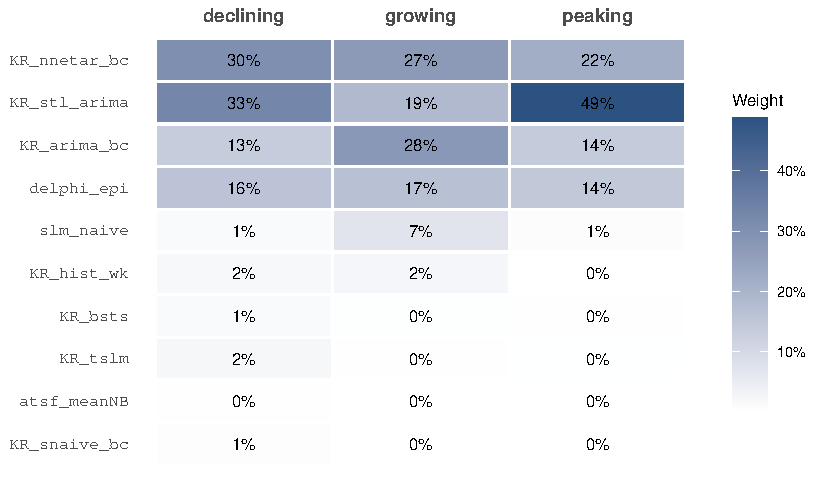
\includegraphics[width=0.85\textwidth]{weights_heatmap.pdf}
\caption{Regime-conditional BMA weights for the 10-model expanded
ensemble. Cells show softmax weights; deeper blue indicates higher
weight. Rows ordered by aggregate validation WIS (best at top).}
\label{fig:weights}
\end{figure}

% =============================================================================
\section{Discussion \& Conclusions}
% =============================================================================

Regime conditioning was the most consequential design choice.
\texttt{stl\_arima\_bc}'s trend-cycle decomposition leads peaking
(49\%) and declining (33\%), the two regimes where the underlying
trend is shifting; the decomposition explicitly models that shift.
\texttt{arima\_bc\_bs} leads growing (28\%), where the trend is
steady and autocorrelation dominates. \texttt{nnetar\_bc\_bs} takes
a stable 22--30\% in every regime, providing competent secondary
skill without specializing. Pool-wide weighting averages these
specializations away. The choice of softmax over direct objective
minimization mattered too: stacking minimizes the validation
objective directly, but the 80 peaking-regime cells were too few
to support its higher-variance fit, and BMA's smoother weights
generalized better. Pool expansion was the smallest of the three
effects: a 2.66\% gain that held only when paired with BMA, since
equal-weight got worse on the same expanded set.

The frozen-weight design assumes validation-period regime patterns
generalize to test seasons. That assumption is challenged by atypical
seasons (2017--18 was unusually severe; 2019--20 was COVID-disrupted),
and an expanding-window BMA could update weights as test-period truth
arrives.

A regime-conditional BMA ensemble on a 10-model diversity-pruned
pool achieved validation LOO total WIS of 614, beating its best
individual component by 13.7\%, equal-weight aggregation by
14--18\%, and leading in every regime. Pool expansion helped BMA
but hurt equal-weight: more candidates help only if the method can
use them.

% =============================================================================
\newpage
\bibliographystyle{plain}
\begin{thebibliography}{9}\small

\bibitem{bracher2021wis}
Bracher J, Ray EL, Gneiting T, Reich NG.
\textit{Evaluating epidemic forecasts in an interval format.}
PLoS Computational Biology 17(2): e1008618, 2021.

\bibitem{bosse2022scoringutils}
Bosse NI, Gruson H, Funk S, Cori A, van Leeuwen E, Abbott S.
\textit{Evaluating Forecasts with scoringutils in R.}
arXiv preprint arXiv:2205.07090, 2022.

\bibitem{scott2014bsts}
Scott SL, Varian HR.
\textit{Predicting the present with Bayesian structural time series.}
International Journal of Mathematical Modelling and Numerical
Optimisation 5(1--2): 4--23, 2014.

\bibitem{delphi2017epicast}
Farrow DC, Brooks LC, Hyun S, Tibshirani RJ, Burke DS, Rosenfeld R.
\textit{A human judgment approach to epidemiological forecasting.}
PLoS Computational Biology 13(3): e1005248, 2017.

\bibitem{ray2023ensemble}
Ray EL, Brooks LC, Bien J, et al.
\textit{Comparing trained and untrained probabilistic ensemble forecasts of COVID-19 cases and deaths in the United States.}
International Journal of Forecasting 39(3): 1366--1383, 2023.

\bibitem{hyndman2021fpp3}
Hyndman RJ, Athanasopoulos G.
\textit{Forecasting: Principles and Practice}, 3rd Edition.
OTexts, 2021. \url{https://otexts.com/fpp3/}.

\end{thebibliography}

\end{document}
